\section*{Appendix - Proofs}
%
%
\begingroup
\def\thetheoremUnified{\ref{lem: monoidal functor Bcirc Bfun}}
\begin{theorem}
  There is a strict monoidal functor $\texttt{ext}: \Bcirc \to \Bfun$ sending
  $I$ to $\Bool^0$, $X$ to $\Bool$, $\NANDSym$ to the usual 
  \texttt{NAND} function $\Bool^2 \to \Bool$, $\COPYSym$ to the 
  cartesian diagonal on $\Bool$, and $\top, \bot$ to the 
  functions $\Bool^0 \to \Bool$ corresponding to the constants 
  $1$ and $0$, respectively.
\end{theorem}
\addtocounter{theoremUnified}{-1}
\endgroup
\begin{proof}
  Strict monoidal functoriality is obvious from the freeness of $\Bcirc$.
\end{proof}
%
%
\begin{lemma}\label{lem: bkp is a bicategory}
  $\Bkp$ as defined in Definition~\ref{def: definition of bkp} is a bicategory.
\end{lemma}
\begin{proof}
  First notice that for each $A,B$, $\Bkp(A,B)$ is trivially a category, 
  since function extensionality is reflexive and transitive.

  Moreover, composition is clearly functorial. This follows from the fact 
  that extensionality is a congruence with respect to function composition.

  The existence of unitors and associators follows from the fact that 
  $\ANDSym(x, 1)$ and $\ANDSym(1,x)$ are extensionally equal to the 
  identity function $\Bool \to \Bool$, as extensionally equal are 
  $\ANDSym(\ANDSym(\_,\_),\_)$ and $\ANDSym(\_,\ANDSym(\_,\_))$.

  Naturality and satisfaction of pentagon and triangle identities for 
  associators and unitors, respectively, follows from the 
  fact that the 2-cell structure of $\Bkp$ is a preorder, so proving 
  that such morphisms exist is enough.
\end{proof}
%
%
\begingroup
\def\thetheoremUnified{\ref{thm: path functor}}
\begin{theorem}
  Having chosen an enumeration on the vertexes and edges of a graph $G$, there 
  is a pseudofunctor $\Free{G} \to \Bkp$, sending 
  each object to $X^V$, and each generating morphism $e$ of $\Free{G}$ to the 
  following morphism, called \emph{$e$-evaluator}, where $e$ represents the 
  constant gate outputting the enumeration of $e$ when considered as an edge of $G$:
  %
  %
  \begin{equation*}
    (\Id{X^V} \Tensor e);(\Id{X^V} \Tensor \COPYSym_{X^E});
      (\Id{X^V} \Tensor S_G \Tensor T_G);(\MATCHSym_{X^V} \Tensor \Id{X^V})
  \end{equation*}
  %
  %
  \begin{equation*}
    \begin{tikzpicture}
      \node[draw, circle, radius=5pt, thick] (copy) at (-1,0.5) {};
      \node[draw, minimum height=20, minimum width=20, rounded corners=2, thick] (S) at (0,1) {$S_G$};
      \node[draw, minimum height=20, minimum width=20, rounded corners=2, thick] (T) at (0,0) {$T_G$};
      \node[draw, fill=gray, circle, radius=5pt, thick] (mat) at (1,1.5) {};

      \node[draw, dashed, minimum height=80, minimum width=110] (contour) at (-0.5,0.8) {};

      \node (Xv) at (-3,2) {$X^V$};
      \node[draw, regular polygon, regular polygon sides = 3, rotate=-30, thick, label={[rotate=4]center:$e$}] (Xe) at (-1.75,0.5) {};
      \node (X) at (2,1.5) {$X$};
      \node (Xv2) at (2,0) {$X^V$};

      \draw[-, thick] (Xv) to (10pt,2);
      \draw[bend left, thick] (10pt,2) to (mat.north);
      \draw[bend right, thick] (S.east) to (mat.south);

      \draw[dashed, -, thick] (Xe) to (copy.west);

      \draw[dashed, bend left, thick] (copy.north) to (S.west);
      \draw[dashed, bend right, thick] (copy.south) to (T.west);

      \draw[-, dotted, thick] (mat.east) -- (X);
      \draw[-, thick] (T.east) -- (Xv2.west);
    \end{tikzpicture}
  \end{equation*}
  %
  %
  The image of $\Free{G}$ through this pseudofunctor is called 
  $\Bpath{G}$, the category of \emph{path proofs over $G$.}
\end{theorem}
\addtocounter{theoremUnified}{-1}
\endgroup
\begin{proof}
  Obvious from the freeness of $\Free{G}$ and the fact that the 
  bicategorical structure of $\Bkp$ is trivial.
\end{proof}
%
%
\begingroup
\def\thetheoremUnified{\ref{thm: path functor}}
\begin{lemma}
  Consider the category $\Count$, which has one object $*$ and 
  natural numbers as morphisms, with $0$ is the identity morphism 
  and composition as addition. 

  For each graph $G$, there is a pseudofunctor $\Free{G} \to \Count$ sending 
  every object to  $*$, identities to $0$, and generating morphisms to $1$.
  This extends to a functorial correspondence between $\Graph$ and the 
  category of endofunctors over $\Count$.
\end{lemma}
\addtocounter{theoremUnified}{-1}
\endgroup
\begin{proof}
  Functoriality is obvious from the freeness of $\Free{G}$.
  Moreover, observe how any morphism of graphs induces a functor between 
  their corresponding free categories which sends generating morphisms 
  to generating morphisms. In particular, this means that such 
  functor preserves the length of paths, making the following diagram 
  trivially commute:
  %
  %
  \begin{equation*}
    \begin{tikzpicture}
      \node (G') at (-2,0) {$G'$}; 
      \node (G) at (-2,2) {$G$};
      \node (FG') at (0,0) {$\Free{G'}$}; 
      \node (FG) at (0,2) {$\Free{G}$};
      \node (Count') at (2,0) {$\Count$};
      \node (Count) at (2,2) {$\Count$};
      \draw[->] (G) -- node[left] {$f$} (G');
      \draw[->] (G) -- (FG);
      \draw[->] (G') -- (FG');
      \draw[->] (FG) -- node[left] {$\Free{f}$} (FG');
      \draw[->] (FG) -- (Count);
      \draw[->] (FG') -- (Count');
      \draw[transform canvas={xshift=-1pt}, -] (Count) -- (Count');
      \draw[transform canvas={xshift=1pt}, -] (Count) -- (Count');
    \end{tikzpicture}
  \end{equation*}
  %
  This suffices to prove the existence of a functorial correspondence $\Graph \to \Cat(\Count, \Count)$.
\end{proof}
%
%
\begingroup
\def\thetheoremUnified{\ref{thm: graph functor}}
\begin{theorem}
  For a graph $G$, consider an enumeration and $S_G$ and $T_G$ 
  as defined in Theorem~\ref{thm: path functor}. There is a pseudofunctor 
  $\Count \to \Bkp$ sending $*$ to $X^V$, $0$ to $\Id{X^V}$ 
  and $n > 0$ to the $n$-fold composition of the morphism
  %
  %
  \begin{equation*}
      (\Id{X^V} \Tensor \COPYSym_{X^E});
      (\Id{X^V} \Tensor S_G \Tensor T_G);(\MATCHSym_{X^V} \Tensor \Id{X^V})
  \end{equation*}
  %
  The composition of this pseudofunctor with the pseudofunctor of 
  Lemma~\ref{lem: functor to count} gives a pseudofunctor 
  $\Free{G} \to \Count \to \Bkp$ sending each object to $X^V$, and each 
  generating morphism to the circuit:
  %
  %
  \begin{equation*}
    (\Id{X^V} \Tensor \COPYSym_{X^E});
      (\Id{X^V} \Tensor S_G \Tensor T_G);(\MATCHSym_{X^V} \Tensor \Id{X^V})
  \end{equation*}
  %
  %
  \begin{equation*}
    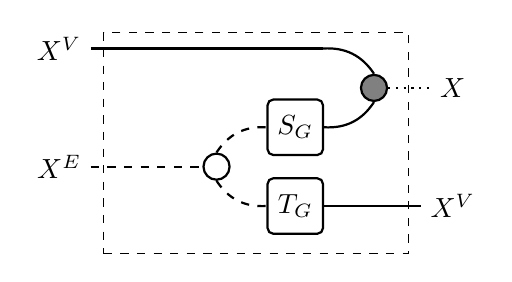
\begin{tikzpicture}
      \node[draw, circle, radius=5pt, thick] (copy) at (-1,0.5) {};
      \node[draw, minimum height=20, minimum width=20, rounded corners=2, thick] (S) at (0,1) {$S_G$};
      \node[draw, minimum height=20, minimum width=20, rounded corners=2, thick] (T) at (0,0) {$T_G$};
      \node[draw, fill=gray, circle, radius=5pt, thick] (mat) at (1,1.5) {};

      \node[draw, dashed, minimum height=80, minimum width=110] (contour) at (-0.5,0.8) {};

      \node (Xv) at (-3,2) {$X^V$};
      \node (Xe) at (-3,0.5) {$X^E$};
      \node (X) at (2,1.5) {$X$};
      \node (Xv2) at (2,0) {$X^V$};

      \draw[-, thick] (Xv) to (10pt,2);
      \draw[bend left, thick] (10pt,2) to (mat.north);
      \draw[bend right, thick] (S.east) to (mat.south);

      \draw[dashed, -, thick] (Xe) to (copy.west);

      \draw[dashed, bend left, thick] (copy.north) to (S.west);
      \draw[dashed, bend right, thick] (copy.south) to (T.west);

      \draw[-, dotted, thick] (mat.east) -- (X);
      \draw[-, thick] (T.east) -- (Xv2.west);
    \end{tikzpicture}
  \end{equation*}
  %
  The image of $\Free{G}$ through this pseudofunctor 
  is called $\Bgraph{G}$, the category of \emph{proofs over $G$.}
\end{theorem}
\addtocounter{theoremUnified}{-1}
\endgroup
\begin{proof}
  The only non-trivial part is proving pseudofunctoriality 
  of the functor $\Count \to \Bkp$. For this, notice that 
  the same natural number $n$ can be obtained by 
  adding smaller numbers in different orders, and with 
  different bracketings. These will in turn correspond to 
  different ways to compose the same morphism in $\Bkp$,
  $n$-times. All these compositions are extensionally equal, 
  which guarantees the existence of isomorphic 2-cells between 
  them. Pseudofunctoriality follows trivially, leveraging on the 
  fact that the 2-cell structure of $\Bkp$ is itself trivial.
\end{proof}
%
%
\begin{lemma}
  For each $n$, $\Bzkp{n}$ as defined in Definition~\ref{def: definition of bzkp} is a bicategory.
\end{lemma}
\begin{proof}
  The proof proceeds exactly as in Lemma~\ref{lem: bkp is a bicategory}, 
  by applying function extensionality also to different 
  compositions of $\COPYSym_X^m$  and $\sigma_{X^{f(n,m)},X^m}$.
\end{proof}
%
%
\begingroup
\def\thetheoremUnified{\ref{thm: the cube}}
\begin{theorem}
  Let $G$, $G'$ be graphs with $n, n'$ vertices and $m, m'$ 
  edges, respectively. Denote with $f(n,m)$ the function 
  outputting how many bits are needed to store the source 
  and target truth tables for graphs with $n$ vertexes and $m$ edges. 
  Then for each morphism $G \to G'$ the following diagram commutes:
  %
\begin{equation*}
  \begin{tikzpicture}
    \pgfdeclarelayer{fg}
    \pgfdeclarelayer{crossing}
    \pgfdeclarelayer{bg}
    \pgfsetlayers{main,bg,crossing,fg}
    %
    \node (G') at (0,0) {$G'$};
    \node(G) at (0,2.25) {$G$};
    \node(FG') at (3,0) {$\Free{G'}$};
    \node(FG) at (3,2.25) {$\Free{G}$};
    \node(Bpath') at (8,0) {$\Bpath{G'}$};
    \node(Bpath) at (8,2.25) {$\Bpath{G}$};
    \node(Count') at (4.5,1.5) {$\Count$};
    \node(Count) at (4.5,3.75) {$\Count$};
    \node(Bzkp') at (6,3) {$\Bzkp{f(m',n')}$};
    \node(Bzkp) at (6,5.25) {$\Bzkp{f(m,n)}$};
    \node(Bgraph') at (9.5,1.5) {$\Bgraph{G'}$};
    \node(Bgraph) at (9.5,3.75) {$\Bgraph{G}$};
    \node(Bzkp1') at (11,3) {$\Bzkp{f(m',n')}$};
    \node(Bzkp1) at (11,5.25) {$\Bzkp{f(m,n)}$};
    % Top
      \draw[->] (G) -- (FG);
      \draw[->] (FG) -- (Count);
      \draw[->] (Count) -- (Bzkp);
      \draw[transform canvas={yshift=-1pt, xshift=-1pt}, =] (Bzkp) -- (Bzkp1);
      \draw[transform canvas={yshift=1pt, xshift=1pt}, =] (Bzkp) -- (Bzkp1);
      \draw[->]  (Bgraph) -- (Bzkp1) ;
    % Bottom
      \draw[->] (G') -- (FG');
      \draw[->] (FG') -- (Bpath');
      \draw[->] (FG') -- (Count');
      \draw[->] (Bgraph') --  (Bzkp1');
      \draw[->] (Bpath') -- (Bgraph');
    % Vertical
      \draw[->] (G) -- (G');
      \draw[->] (FG) -- (FG');
      \draw[->] (Bzkp1) -- (Bzkp1');
    %FG
    \begin{pgfonlayer}{fg}
      \draw[->, name path global/.expanded=fgbpath] (FG) -- (Bpath);
      \draw[->, name path global/.expanded=countbgraph] (Count) -- (Bgraph);
      \draw[->, name path global/.expanded=bgraphbpath] (Bpath) -- (Bgraph);
      \draw[->, name path global/.expanded = bgraphbgraph'] (Bgraph) -- (Bgraph');
      \draw[->, name path global/.expanded=bpathbpath'] (Bpath) -- (Bpath');
    \end{pgfonlayer}
  %BG
    \begin{pgfonlayer}{bg}
      \draw[-> , name path global/.expanded=countbzkp'] (Count') -- (Bzkp');
      \draw[->, name path global/.expanded=countbgraph'] (Count') -- (Bgraph');
      \draw[transform canvas={yshift=-1pt, xshift=-1pt}, =, name path global/.expanded=bzkpid1] (Bzkp') -- (Bzkp1');
      \draw[transform canvas={yshift=1pt, xshift=1pt}, =, name path global/.expanded=bzkpid2] (Bzkp') -- (Bzkp1');
      \draw[transform canvas={xshift=-1pt}, =, name path global/.expanded=countcount'1] (Count) -- (Count');
      \draw[transform canvas={xshift=1pt}, =, name path global/.expanded=countcount'2] (Count) -- (Count');
      \draw[->, name path=bzkpbzkp'] (Bzkp) -- (Bzkp');
    \end{pgfonlayer}
    % Intersections
    \begin{pgfonlayer}{crossing}
      \fill[white, name intersections={of=bgraphbpath and bzkpid1, name=i}] (i-1) circle (3pt);
      \fill[white, name intersections={of=bgraphbpath and bzkpid2, name=i}] (i-1) circle (3pt);
      \fill[white, name intersections={of=bgraphbgraph' and bzkpid1, name=i}] (i-1) circle (3pt);
      \fill[white, name intersections={of=bgraphbgraph' and bzkpid2, name=i}] (i-1) circle (3pt);
      \fill[white, name intersections={of=fgbpath and countbzkp', name=i}] (i-1) circle (3pt);
      \fill[white, name intersections={of=countbgraph' and bpathbpath', name=i}] (i-1) circle (3pt);
      \fill[white, name intersections={of=bzkpbzkp' and countbgraph, name=i}] (i-1) circle (3pt);
      \fill[white, name intersections={of=countcount'1 and fgbpath, name=i}] (i-1) circle (3pt);
      \fill[white, name intersections={of=countcount'2 and fgbpath, name=i}] (i-1) circle (3pt);
    \end{pgfonlayer}
    %
    \end{tikzpicture}
  %
\end{equation*}
%
\end{theorem}
\addtocounter{theoremUnified}{-1}
\endgroup
\begin{proof}
  We will prove the commutativity of single squares, 
  starting from the top face. In the square:
  %
  %
  \begin{equation*}
    \begin{tikzpicture}
      \node (FG) at (0,0) {$\Free{G}$}; 
      \node (Count) at (0,2) {$\Count$};
      \node (BpathG) at (2,0) {$\Bpath{G}$}; 
      \node (BgraphG) at (2,2) {$\Bgraph{G}$};
      \draw[->] (FG) -- (Count);
      \draw[->] (Count) -- (BgraphG);
      \draw[->] (FG) -- (BpathG);
      \draw[->] (BpathG) -- (BgraphG);
    \end{tikzpicture}
  \end{equation*}
  % 
  We notice that the bottom functor acts by sending 
  each edge $e$ to the morphism:
  %
  %
  \begin{equation*}
    (\Id{X^n} \Tensor e);(\Id{X^n} \Tensor \COPYSym_{X^m});
    (\Id{X^n} \Tensor S_G \Tensor T_G);(\MATCHSym_{X^n} \Tensor \Id{X^n})
  \end{equation*}
  %
  Being a subcategory of $\Bcirc$, which is free symmetric monoidal,
  eavery morphism in $\Bpath{G}$ is just a composition of a finite 
  number of morphisms as the one above for some edges $e_1, \dots, e_n$.
  We then define a pseudofunctor sending each morphism 
    %
  %
  \begin{equation*}
    (\Id{X^n} \Tensor e);(\Id{X^n} \Tensor \COPYSym_{X^m});
    (\Id{X^n} \Tensor S_G \Tensor T_G);(\MATCHSym_{X^n} \Tensor \Id{X^n})
  \end{equation*}
  %
  To:
  %
  %
  \begin{equation*}
    (\Id{X^n} \Tensor \COPYSym_{X^m});
    (\Id{X^n} \Tensor S_G \Tensor T_G);(\MATCHSym_{X^n} \Tensor \Id{X^n})
  \end{equation*}
  %
  The mapping on 2-cells is trivial. Pseudofunctoriality 
  is obvious and follows from function extensionality
  being a congruence wrt function composition. Commutativity 
  is obvious too since the morphism above is precisely where
  precisely where each generating morphism in $\Free{G}$ gets sent to
  when going through $\Count$.

  The square:
  %
  %
  \begin{equation*}
    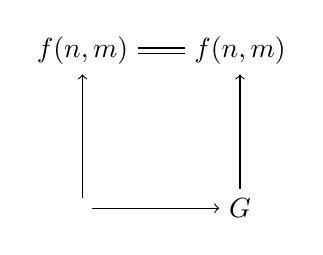
\begin{tikzpicture}
      \node (Count) at (0,0) {$\Count$};
      \node (BgraphG) at (2,0) {$\Bgraph{G}$};
      \node (BpathG) at (2,2) {$\Bzkp{f(n,m)}$}; 
      \node (FG) at (0,2) {$\Bzkp{f(n,m)}$}; 

      \draw[<-] (FG) -- (Count);
      \draw[->] (Count) -- (BgraphG);
      \draw[transform canvas={yshift=-1pt}, =] (FG) -- (BpathG);
      \draw[transform canvas={yshift=1pt}, =] (FG) -- (BpathG);
      \draw[<-] (BpathG) -- (BgraphG);
    \end{tikzpicture}
  \end{equation*}
  % 
  Commutes by noticing that $\Bgraph{G}$ is again generated by the morphism 
  %
  %
  \begin{equation*}
    (\Id{X^n} \Tensor \COPYSym_{X^m});
    (\Id{X^n} \Tensor S_G \Tensor T_G);(\MATCHSym_{X^n} \Tensor \Id{X^n})
  \end{equation*}
  %
   We can then define the right-edge pseudofunctor to be sending it to:
  %
  %
  \begin{equation*}
    (\Id{X^n} \Tensor \COPYSym_{X^{f(n,m)}} \Tensor \COPYSym_{X^m});
    (\Id{X^n \Tensor X^{f(n,m)}} \Tensor \sigma_{X^{f(n,m)},X^m} \Tensor \Id{X^m});
    (\Id{X^n} \Tensor S_{n,m} \Tensor T_{n,m});(\MATCHSym_{X^n} \Tensor \Id{X^n})
  \end{equation*}
  %
  %
  The mapping on 2-cells is again trivial. 
  Pseudofunctoriality  and square commutativity 
  follow as in the previous case.

  The bottom face is equal to the top one, so we now switch to 
  the side faces. Consider a graph morphism $g:G \to G'$.
  Commutativity of 
  %
  %
  \begin{equation*}
    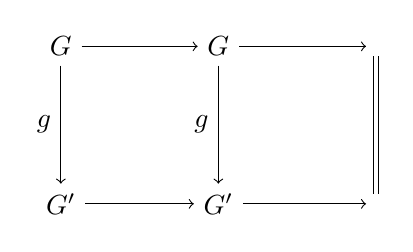
\begin{tikzpicture}
      \node (G') at (-2,0) {$G'$}; 
      \node (G) at (-2,2) {$G$};
      \node (FG') at (0,0) {$\Free{G'}$}; 
      \node (FG) at (0,2) {$\Free{G}$};
      \node (Count') at (2,0) {$\Count$};
      \node (Count) at (2,2) {$\Count$};
      \draw[->] (G) -- node[left] {$g$} (G');
      \draw[->] (G) -- (FG);
      \draw[->] (G') -- (FG');
      \draw[->] (FG) -- node[left] {$\Free{g}$} (FG');
      \draw[->] (FG) -- (Count);
      \draw[->] (FG') -- (Count');
      \draw[transform canvas={xshift=-1pt}, -] (Count) -- (Count');
      \draw[transform canvas={xshift=1pt}, -] (Count) -- (Count');
    \end{tikzpicture}
  \end{equation*}
  %
  Is just Lemma~\ref{lem: functor to count}. As for the square:
  %
  %
  \begin{equation*}
    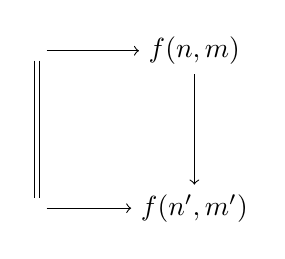
\begin{tikzpicture}
      \node (Count) at (0,2) {$\Count$};
      \node (Count') at (0,0) {$\Count$};
      \node (Bzkp) at (2,2) {$\Bzkp{f(n,m)}$}; 
      \node (Bzkp') at (2,0) {$\Bzkp{f(n',m')}$}; 
      \draw[->] (Count) -- (Bzkp);
      \draw[->] (Count') -- (Bzkp');
      \draw[->] (Bzkp) -- (Bzkp');
      \draw[transform canvas={xshift=-1pt}, -] (Count) -- (Count');
      \draw[transform canvas={xshift=1pt}, -] (Count) -- (Count');
    \end{tikzpicture}
  \end{equation*}
  %
  It is sufficient to define the pseudofunctor 
  $\Bzkp{f(n,m)} \to \Bzkp{f(n', m')}$ as sending 
  $X^n$ to $X^{n'}$, and the generating morphism
  %
  %
  \begin{equation*}
    (\Id{X^n} \Tensor \COPYSym_{X^{f(n,m)}} \Tensor \COPYSym_{X^m});
    (\Id{X^n \Tensor X^{f(n,m)}} \Tensor \sigma_{X^{f(n,m)},X^m} \Tensor \Id{X^m});
    (\Id{X^n} \Tensor S_{n,m} \Tensor T_{n,m});(\MATCHSym_{X^n} \Tensor \Id{X^n})
  \end{equation*}
  %
  To:
  %
  %
  \small{
  \begin{equation*}
    (\Id{X^{n'}} \Tensor \COPYSym_{X^{f(n',m')}} \Tensor \COPYSym_{X^{m'}});
    (\Id{X^{n'} \Tensor X^{f(n',m')}} \Tensor \sigma_{X^{f(n',m')},X^{m'}} \Tensor \Id{X^{m'}});
    (\Id{X^{n'}} \Tensor S_{n',m'} \Tensor T_{n',m'});(\MATCHSym_{X^{n'}} \Tensor \Id{X^{n'}})
  \end{equation*}}
  %
  According to this definition extensionally equal circuits 
  are sent to extensionally equal circuits, so 2-cells can be 
  defined in the obvious way. Commutativity of the square 
  is again true by definition. A slight modification of the 
  proof above allows us to also prove the commutativity
  of the following square:
  %
  %
  \begin{equation*}
    \begin{tikzpicture}
      \node (Count) at (0,2) {$\Count$};
      \node (Count') at (0,0) {$\Count$};
      \node (Bzkp) at (2,2) {$\Bgraph{G}$}; 
      \node (Bzkp') at (2,0) {$\Bgraph{G'}$}; 
      \draw[->] (Count) -- (Bzkp);
      \draw[->] (Count') -- (Bzkp');
      \draw[->] (Bzkp) -- (Bzkp');
      \draw[transform canvas={xshift=-1pt}, -] (Count) -- (Count');
      \draw[transform canvas={xshift=1pt}, -] (Count) -- (Count');
    \end{tikzpicture}
  \end{equation*}
  %
  Now we focus on:
  %
  %
  \begin{equation*}
    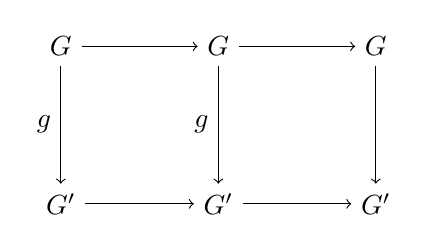
\begin{tikzpicture}
      \node (G') at (-2,0) {$G'$}; 
      \node (G) at (-2,2) {$G$};
      \node (FG') at (0,0) {$\Free{G'}$}; 
      \node (FG) at (0,2) {$\Free{G}$};
      \node (Bpath') at (2,0) {$\Bpath{G'}$};
      \node (Bpath) at (2,2) {$\Bpath{G}$};
      \draw[->] (G) -- node[left] {$g$} (G');
      \draw[->] (G) -- (FG);
      \draw[->] (G') -- (FG');
      \draw[->] (FG) -- node[left] {$\Free{g}$} (FG');
      \draw[->] (FG) -- (Bpath);
      \draw[->] (FG') -- (Bpath');
      \draw[->] (Bpath) -- (Bpath');
    \end{tikzpicture}
  \end{equation*}
  %
  Whose commutativity is obvious by defining the 
  pseudofunctor $\Bpath{G} \to \Bpath{G'}$ by sending 
  $X^n$ to $X^{n'}$, and every morpsism
  %
  %
  \begin{equation*}
    (\Id{X^n} \Tensor e);(\Id{X^n} \Tensor \COPYSym_{X^m});
    (\Id{X^n} \Tensor S_G \Tensor T_G);(\MATCHSym_{X^n} \Tensor \Id{X^n})
  \end{equation*}
  %
  To:
  %
  %
  \begin{equation*}
    (\Id{X^{n'}} \Tensor \Free{g}(e));(\Id{X^{n'}} \Tensor \COPYSym_{X^{m'}});
    (\Id{X^{n'}} \Tensor S_G \Tensor T_G);(\MATCHSym_{X^{n'}} \Tensor \Id{X^{n'}})
  \end{equation*}
  %
  2-cells mapping is again obvious.

  Finally, we focus on the squares:
  %
  %
  \begin{equation*}
    \begin{tikzpicture}
      \node (Bpath) at (0,2) {$\Bpath{G}$};
      \node (Bpath') at (0,0) {$\Bpath{G'}$};
      \node (Bgraph) at (2,2) {$\Bgraph{G}$}; 
      \node (Bgraph') at (2,0) {$\Bgraph{G'}$}; 
      \draw[->] (Bpath) -- (Bgraph);
      \draw[->] (Bpath') -- (Bgraph');
      \draw[->] (Bgraph) -- (Bgraph');
      \draw[->] (Bpath) -- (Bpath');
    \end{tikzpicture}
    \qquad
    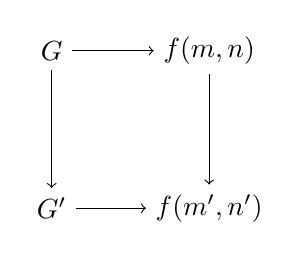
\begin{tikzpicture}
      \node (Bgraph) at (0,2) {$\Bgraph{G}$};
      \node (Bgraph') at (0,0) {$\Bgraph{G'}$};
      \node (Bzkp) at (2,2) {$\Bzkp{f(m,n)}$}; 
      \node (Bzkp') at (2,0) {$\Bzkp{f(m',n')}$}; 
      \draw[->] (Bgraph) -- (Bzkp);
      \draw[->] (Bgraph') -- (Bzkp');
      \draw[->] (Bzkp) -- (Bzkp');
      \draw[->] (Bgraph) -- (Bgraph');
    \end{tikzpicture}
  \end{equation*}
  %
  Whose commutativity is proven similarly. 
  All pseudofunctors involved in these squares 
  have already been defined previously. Commutativity 
  is obvious by tracking where generating morphisms get 
  mapped.
\end{proof} 